\subsection{Comparing Planet Yields from all Extended Missions}
\label{sec:results_from_all_extended_missions}
To compare Extended Missions in terms of planet detection statistics, we focus on the subset of all detected planets that are \textit{newly} detected from each Extended Mission.
These may come from stars that were not observed at all in the Primary Mission (notably for scenarios such as \elong), or they may also come from transiting planets that were observed in the Primary Mission with $\mathrm{SNR}<7.3$, or from planets that were single-transiters in the Primary Mission (we require $N_\mathrm{tra}\geq2$) for detection.
With this in mind, for each Extended Mission scenario we ask the following questions:

\begin{enumerate}
	\item $N_\mathrm{new}$: How many new planets do we detect?
	\item $N_\mathrm{new,P>20d}$: How many of these new planets have periods $>20$ days?
	\item $N_\mathrm{new,HZ}$: How many are in the habitable zone?
	\item $N_\mathrm{sys,extra\ planets}$: In how many systems in which at least one planet was detected during the Primary Mission do we find extra planets in the Extended Mission?
	\item $N_\mathrm{new,atm}$: How many new planets do we find that are amenable to atmospheric characterization (defined below by Eq.~\ref{eq:atmosphere_Deming})?
	\item $N_\mathrm{new,new\ stars}$: How many of the new planets come from 
	stars that were not observed in the Primary Mission? 
	\item $N_\mathrm{new,SNR\lor N_{tra}}$: How many of the new planets come 
	from candidates that after the Primary Mission had either a) 
	$\mathrm{SNR}<7.3$ and/or b) less than 2 transits?
\end{enumerate}
\begin{figure}[!t]
	\centering
	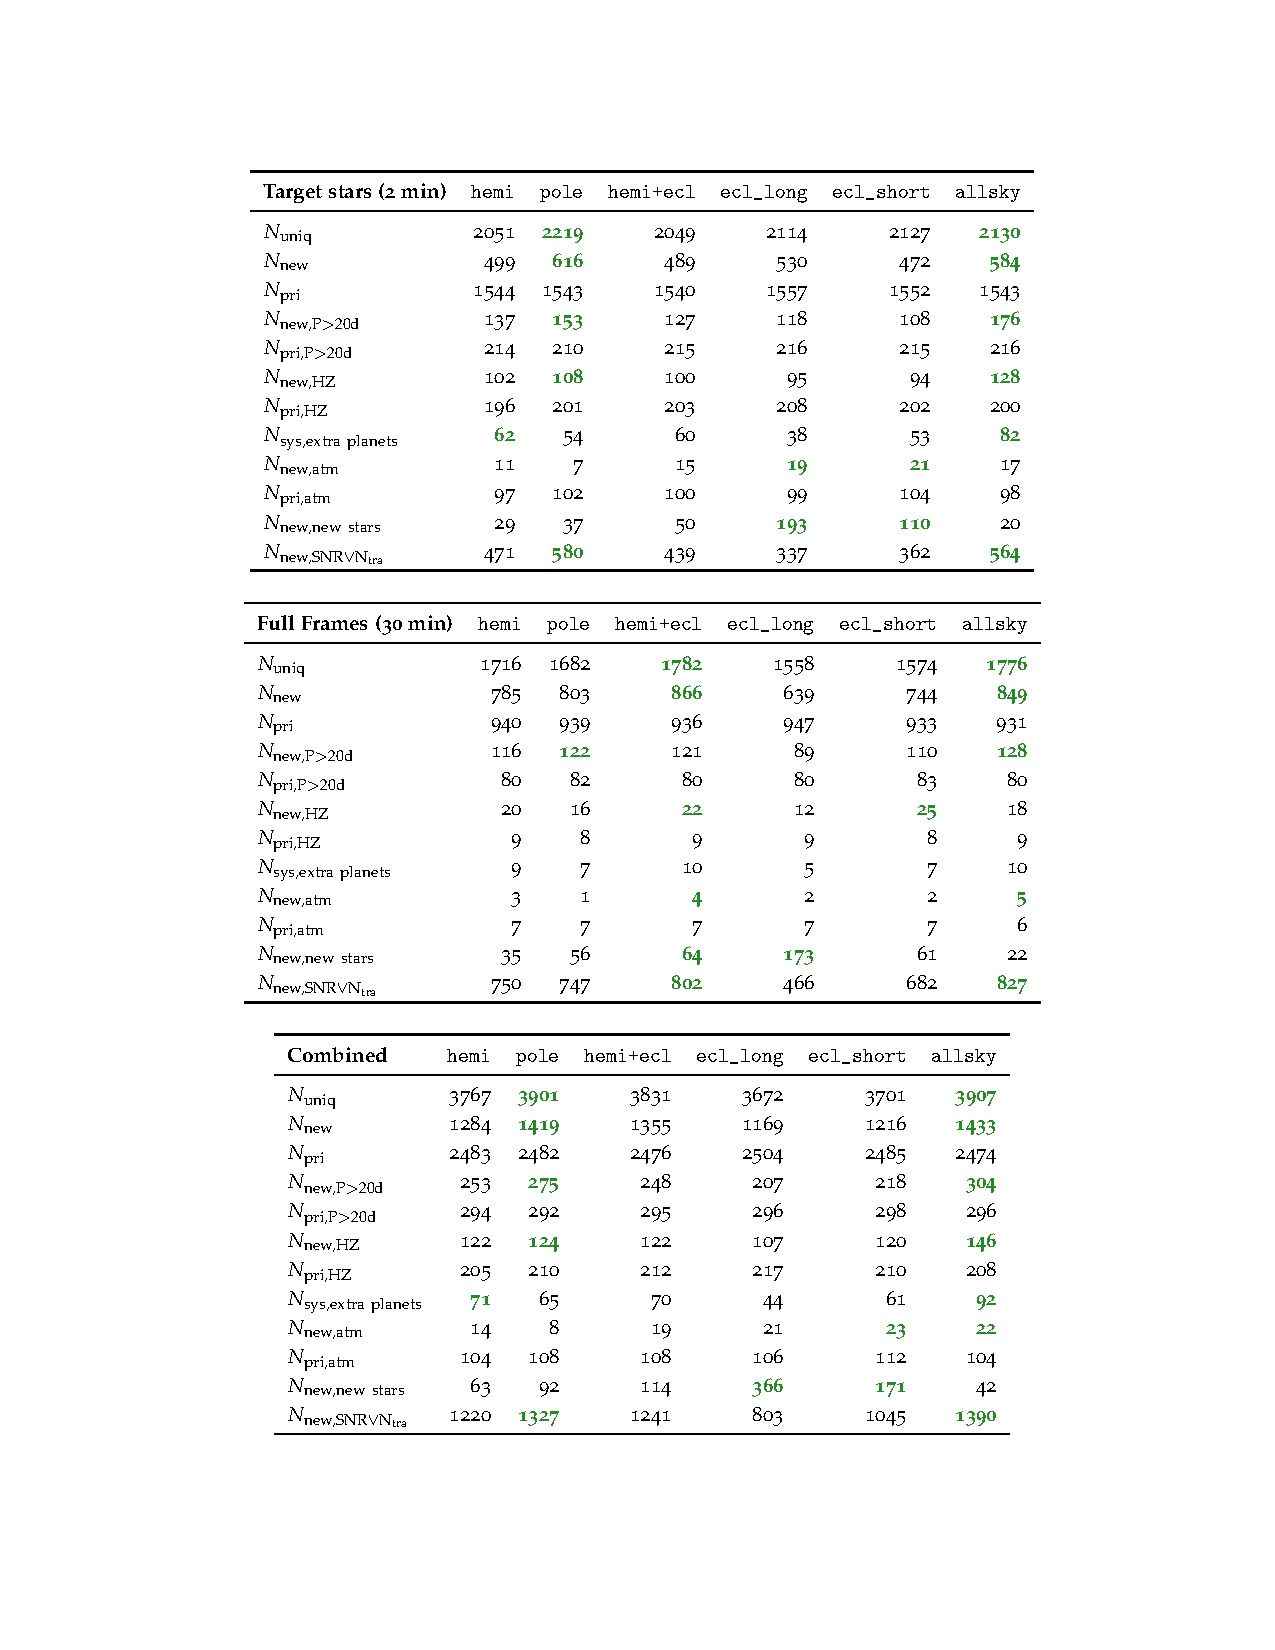
\includegraphics[scale=2.]{tables/cropped_tables_vis_nogap.pdf}
	%from 160729_t50 data. generate with tables_vis.tex
	\caption{Detected planet metrics for six possible Extended Missions (values are means of 50 Monte Carlo realizations of our calculation, all for $R_p<4R_\oplus$).
	\textit{Top:} postage stamp detections, \textit{Middle:} full frame image only detections, \textit{Bottom:} sum of both.
	The best two scenarios for select statistics are bolded and highlighted in 
	green.
	\newline
	$N_\mathrm{uniq}$: number of unique planets detected over all 3 years.
	$N_\mathrm{new}$: number of planets detected in year 3 that were not detected in years 1\&2 (newly detected planets).
	$N_\mathrm{pri}$: number of planets detected in the Primary Mission (years 1\&2).
	$N_\mathrm{new,P>20d}$: number of newly detected planets with orbital periods greater than 20 days.
	$N_\mathrm{pri,P>20d}$: same as previous, but from the Primary Mission.
	$N_\mathrm{new,HZ}$: number of newly detected planets satisfying $0.2<S/S_\oplus<2.0$ (approximate habitable zone).
	$N_\mathrm{pri,HZ}$: same as previous, from the Primary Mission.
	$N_\mathrm{sys,extra\ planets}$: number of systems in which extra planets are detected.
	$N_\mathrm{new,atm}$: number of newly detected planets with SNR in transmission greater than (that of GJ 1214b)/2, as measured by \jwst\,-- see text.
	$N_\mathrm{pri,atm}$: same as previous, from Primary Mission.
	$N_\mathrm{new,new\ stars}$: number of newly detected planets that orbit 
	stars that were not observed during the Primary Mission.
	$N_\mathrm{new,SNR\lor N_{tra}}$: number of newly detected planets that were 
	observed during the Primary Mission, but either (a) had 
	$\mathrm{SNR}<7.3$ and/or b) had $N_\mathrm{tra}<2$, and so would not be 
	`detected'.}
	\label{fig:yield_results}
\end{figure}

For each Year-3 scenario, we compare these numbers to the
corresponding numbers from the Primary Mission as well as to the other
5 scenarios for Year 3. We show the results of our simulations in
Fig.~\ref{fig:yield_results}.  The first point to notice is that for
all but one of the new planet detection metrics ($N_\mathrm{new}$,
$N_\mathrm{new,P>20d}$, $N_\mathrm{new,HZ}$,
$N_\mathrm{sys,extra\ planets}$, $N_\mathrm{new,atm}$,
$N_\mathrm{new,SNR\lor N_{tra}}$) the yields between Extended Missions
vary by less than a factor of two.  The exception is in
$N_\mathrm{new,new\ stars}$, in which \elong\:detects roughly twice as
many planets orbiting never-before-observed stars as any other
proposed mission.

The second point is on the absolute yields of new planets: postage stamp observations find $\mathcal{O}(500)$ new planets, relative to the Primary Mission's $\mathcal{O}(1500)$.
Full frame image observations find $\mathcal{O}(800)$ new planets, relative to the Primary Mission's $\mathcal{O}(900)$.
All Extended Missions find $\mathcal{O}(1300)$ new planets, relative to the Primary Mission's $\mathcal{O}(2500)$.
We discuss these results -- the rough invariance of the number of new planets to different pointing scenarios, and the essential contribution of FFIs -- further in point \#1 below.

Skimming the bottom panel for which missions are highlighted in green when accounting for both PSs and FFIs, we see that \npole\:and \hemis\:are the `superlative-winning' missions in terms of detected planet statistics: considering both PSs and FFIs, \npole\:places top-2 in 5 of 8 relevant categories, and \hemis\:does the same in 6 of 8.
They both do well at maximizing the number of newly detected planets, while also performing well at detecting long period planets, and thus planets in their stars' habitable zones.
\hemis\:also has the largest number of systems in which extra planets are detected.

We now discuss each metric of Fig.~\ref{fig:yield_results} in more depth:
	\begin{figure}[!t]
		\centering
		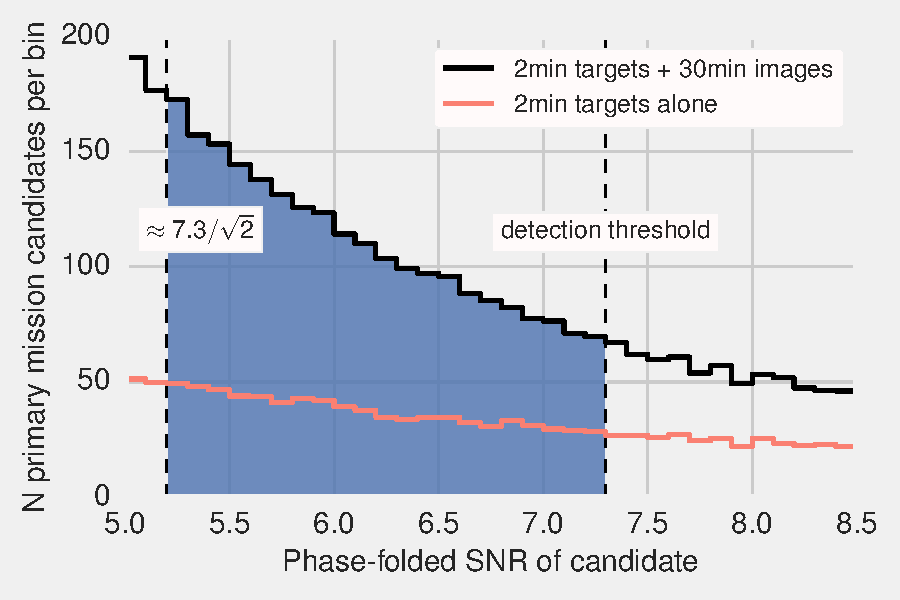
\includegraphics[scale=1.]{figures/snrf_histogram_with_ps.pdf}
		\caption{Histogram of phase-folded SNRs for candidate $R_p<4R_\oplus$ 
			planets following the Primary Mission (from both PS and FFI 
			observations; values are means of 20 Monte Carlo trials; 
			$N_\mathrm{tra}\geq2$).
			If an Extended Mission observes half of the sky, it roughly doubles 
			the number of observed transits for half of the planets observed in 
			the Primary Mission, enabling detection of $\approx 2316/2 = 1158$ 
			planets (half of the blue integrated area in the plot). This coarse 
			estimate is a similar result to our detailed calculations, and 
			shows the value of continuing \tesss observations 
			\textit{irrespective of where we observe}.}
		\label{fig:snrf_histogram}
	\end{figure}
\begin{enumerate}
	\item $N_\mathrm{new}$: we detect about as many new planets in Year 3 as we detect planets in either Years 1 or 2: roughly $1250$.
	The worst and the best scenarios (\elong\:and \hemis, respectively) differ 
	only by a factor of 1.2.
	The fact that there are so many new planets to be detected from extended 
	observations, particularly from full frame images, and that the absolute 
	number of new planets does not depend strongly on the schedule of pointings,
	can be justified (post-facto) with Fig.~\ref{fig:snrf_histogram}.
	This figure illustrates a point that was originally noted by~\citetalias{Sullivan_2015}:
        \tesss Primary Mission will miss many short-period planets around bright stars, and is therefore
        incomplete even in its intended hunting ground.
        For stars with $I_c<11$, there are $\sim\! 10\times$ more transiting 
        $2<R_p<4R_\oplus$ planets on $P<20\,\mathrm{day}$ orbital periods than 
        \tess will detect in its first two years\footnote{Fig 22
        of~\citetalias{Sullivan_2015}; only considers $R_\star<1.5R_\odot$ 
        stars}.
        \citetalias{Sullivan_2015} similarly note that there are $\sim\! 
        20\times$ more transiting $R_p<2R_\oplus$ ($P<20\,\mathrm{day}$, 
        $I_c<11$ host star) planets in the sky than \tess will discover in 
        its Primary Mission.
	Our findings agree: there are a substantial number of planets just below the detection threshold, predominantly with $2R_\oplus < R_p <4R_\oplus$ (Fig.~\ref{fig:primary_planet_yield}).
	An Extended Mission will probe and detect this population, in any of the scenarios we investigate.
	This result should hold equally well for realistic detection efficiency 
	thresholds, and it demonstrates that extended observations will be valuable 
	because \tess will not yet have detected all the planets in the parameter 
	space of $R_p<4R_\oplus$ planets orbiting bright stars on short-period 
	orbits;
	there will still be small, short-period planets orbiting bright stars to 
	be discovered after \tesss Primary Mission.


	\item $N_\mathrm{new,P>20d}$: it will be possible to detect as many new 
	$P>20$ day planets in one year of \tesss Extended Mission as in both years 
	of the Primary Mission.
	The Primary Mission detects about 295 such planets; \hemis\:and 
	\npole\:scenarios detect similar numbers.
	These two scenarios are achieving the goal of long-period planet detection 
	in slightly different ways: % (see discussion in Sec.~\ref{sec:discussion}):
	\npole\:maximizes the average observing baseline per star, while 
	\hemis\:observes the greatest possible number of stars for longer than 40 
	days.
	The latter approach could succeed at detecting many planets (our result is 
	that \hemis\:detects the most $P>20$ day planets), but it relies heavily 
	upon the assumption that we can detect planets from only two transits over 
	the course of the entire mission, even if this means only one transit in 
	the Primary, and one transit in the Extended.
	\begin{figure}[!t]
		\centering
		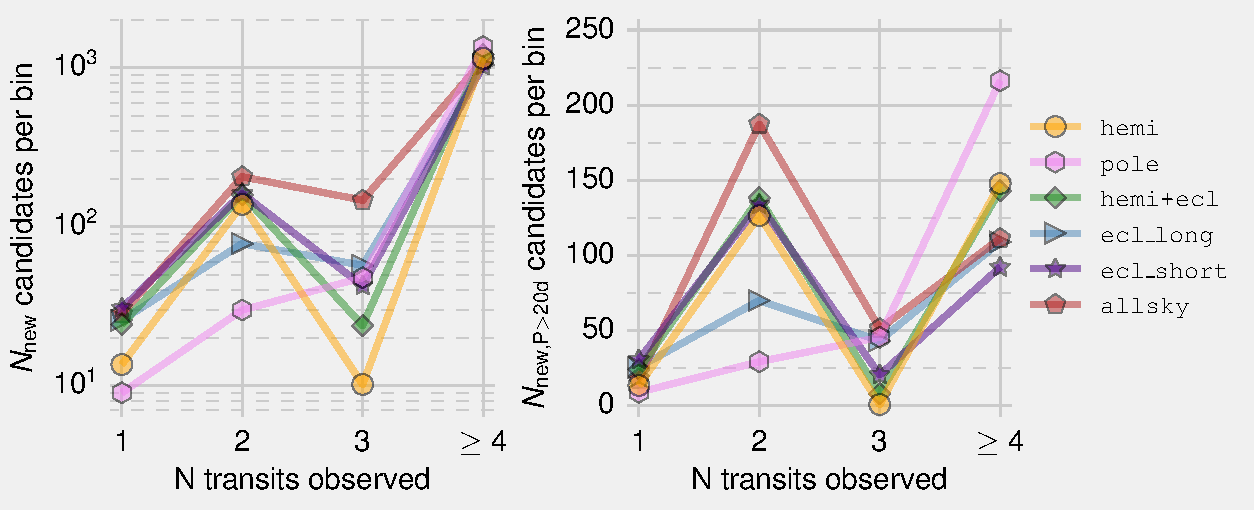
\includegraphics{figures/Ntra_histogram_nogap.pdf}
		%this figure uses 160802 data, which should be the same as 
		%160728_t50, but has ntra_min set to 1 in yieldCode. Read my notes 
		%from ext_sim_notes on this -- something's a bit off with the 
		%normalization. That said, rather than redo the previous figures 
		%with a code that might have a minor bug, my point here -- which is 
		%the hemis14d has this issue with few-transit detections -- isn't 
		%really any different.
		\caption{ \textit{Left:} Histogram of new $R_p<4R_\oplus$ planet 
			candidates from each Extended Mission as a function of the 
			total number of 
			observed transits over all 3 years.
			Planet candidates are `detected' if $N_\mathrm{tra}\geq2$ 
			(see Eq.~\protect\ref{eq:detection_criterion}).
			\textit{Right:} Same as left, restricted to $P>20$ day planets.
			If any given scenario has a `bump' at 2 observed transits, then 
			that scenario depends more heavily on our assumption of being 
			able to make detections based on only two transits.
			Lines joining points have no physical meaning; they are 
			intended to improve readability.}
		\label{fig:Ntra_hist}
	\end{figure}
	\begin{marginfigure}[-1in]
		\centering
		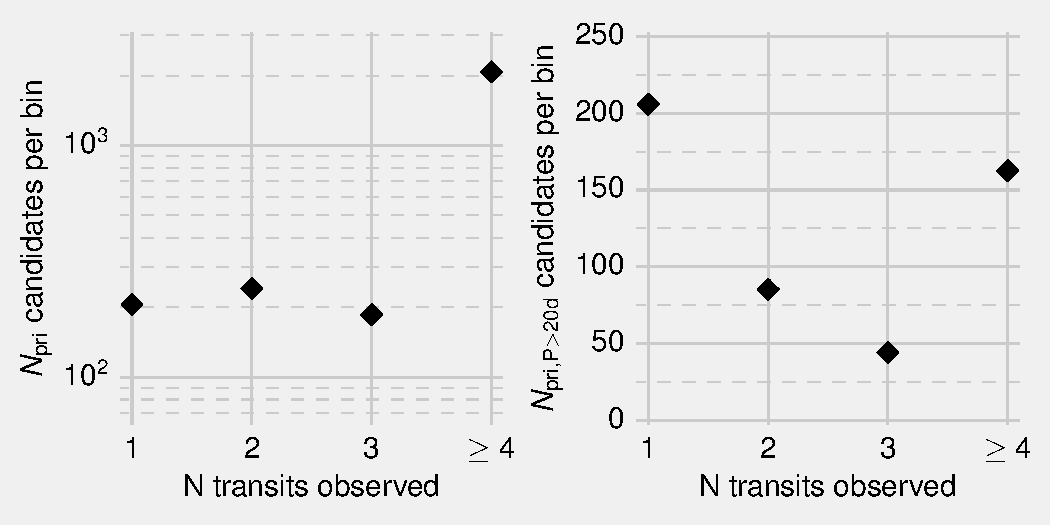
\includegraphics[scale=1.]{figures/Ntra_histogram_primary.pdf}
		%\missingfigure{histogram of Primary Mission number of transits for 
		%detected planets}
		% this figure uses BLAH data
		\caption{ 
			Similar to Fig.~\protect\ref{fig:Ntra_hist}, but for the Primary 
			Mission.
		}
		\label{fig:Ntra_hist_primary}
	\end{marginfigure}
	\vspace{-0.47cm}
	This point -- that the ability of the \hemis\:scenario to detect many long 
	period planets is grounded on the assumption that two transits at high 
	enough SNR are sufficient for detection -- is made explicit in the right 
	panel of Fig.~\ref{fig:Ntra_hist}.
	About half of the long period planets that \hemis\:finds are detected with only two transits.
	By way of comparison, \npole\:detects most of its long-period planets with $\ge 4$ transits.
	This means that the \npole\:detections are more secure.
	For two-transit detections, especially those separated by a gap of a year or more in the \tess data, it will be
        difficult to be confident in either the detection or in the derived 
        orbital period.
    Experience from the \kepler mission showed that requiring 3 or more 
    self-consistent transits substantially lowers the fraction of false 
    signals~\citep{burke_Q1Q8_2014}.
	If we restrict `detections' to planets with both $N_\mathrm{tra}\geq 3$ and 
	$\mathrm{SNR_{phase-folded} \geq 7.3}$, we find that \npole\:detects 
	$\sim\!260$ new long-period planets, while the next-best scenarios, \hemis,
	\nhemi, and \shemiAvoid, all detect about 160.
	
	

	\item $N_\mathrm{new,HZ}$: we approximate the habitable zone as the geometric shell around a host star in which a planet's insolation satisfies $0.2>S/S_\oplus>2.0$.
	With this approximation, the \hemis\:scenario finds the most new habitable zone planets: 146 (which is subject to the same caveats discussed above for long period planet detections). 
	The next-best scenarios, \npole, \npole\:and \shemiAvoid, all detect around 120.
	Relative to the Primary Mission's 210 detections, this means Extended Missions boost the number of detected habitable zone planets by a factor of $\sim1.6$.
	For purposes of weighing the value of habitable-zone detections in deciding 
	between missions, the result that these scenarios all detect a similar 
	number of HZ planets indicates that this metric will likely not `tip the 
	scales' in any direction.
	
	We note in passing that $\sim\!80\%$ of the habitable zone planets that \tess detects orbit M dwarfs with spectral classes ranging from M4 - M0, and $\sim\!15\%$ of them orbit M dwarfs later than M4.
	We show the relevant cumulative distribution in Fig.~\ref{fig:CDF_habitable_zone}.
	% see hz_primary_george/CDF_most_HZ_planets_orbit_early_M_dwarfs.png
	Additionally, our values for the number of $0.2<S/S_\oplus<2$ planets from the Primary Mission are slightly revised from those of~\citetalias{Sullivan_2015}: while~\citetalias{Sullivan_2015} found $48\pm7$ planets with $0.2<S/S_\oplus<2$ and $R_p<2R_\oplus$, we find $34 \pm 5$ such planets.
	Adopting the habitable zone of~\citet{kopparapu_habitable_2013},~\citetalias{Sullivan_2015} found $14\pm4$ planets with $R_p<2R_\oplus$. We find $11 \pm 3$ such planets.
	The rule of thumb that Extended Missions give roughly $1.6\times$ the number of new $0.2<S/S_\oplus<2$ habitable zone planets applies to the~\citet{kopparapu_habitable_2013} habitable zone as well as $0.2<S/S_\oplus<2.0$.
	Another point raised by Fig.~\ref{fig:scatter_habitable_zone} is that the~\citet{kopparapu_habitable_2013} habitable zone, which is physically motivated by 1-D radiative-convective cloud-free climate models with accurate absorption coefficients, results in roughly 3 times fewer `habitable zone' planet detections than our ad-hoc criterion of $0.2<S/S_\oplus<2$.
	\begin{marginfigure}[-5in]
		\centering
		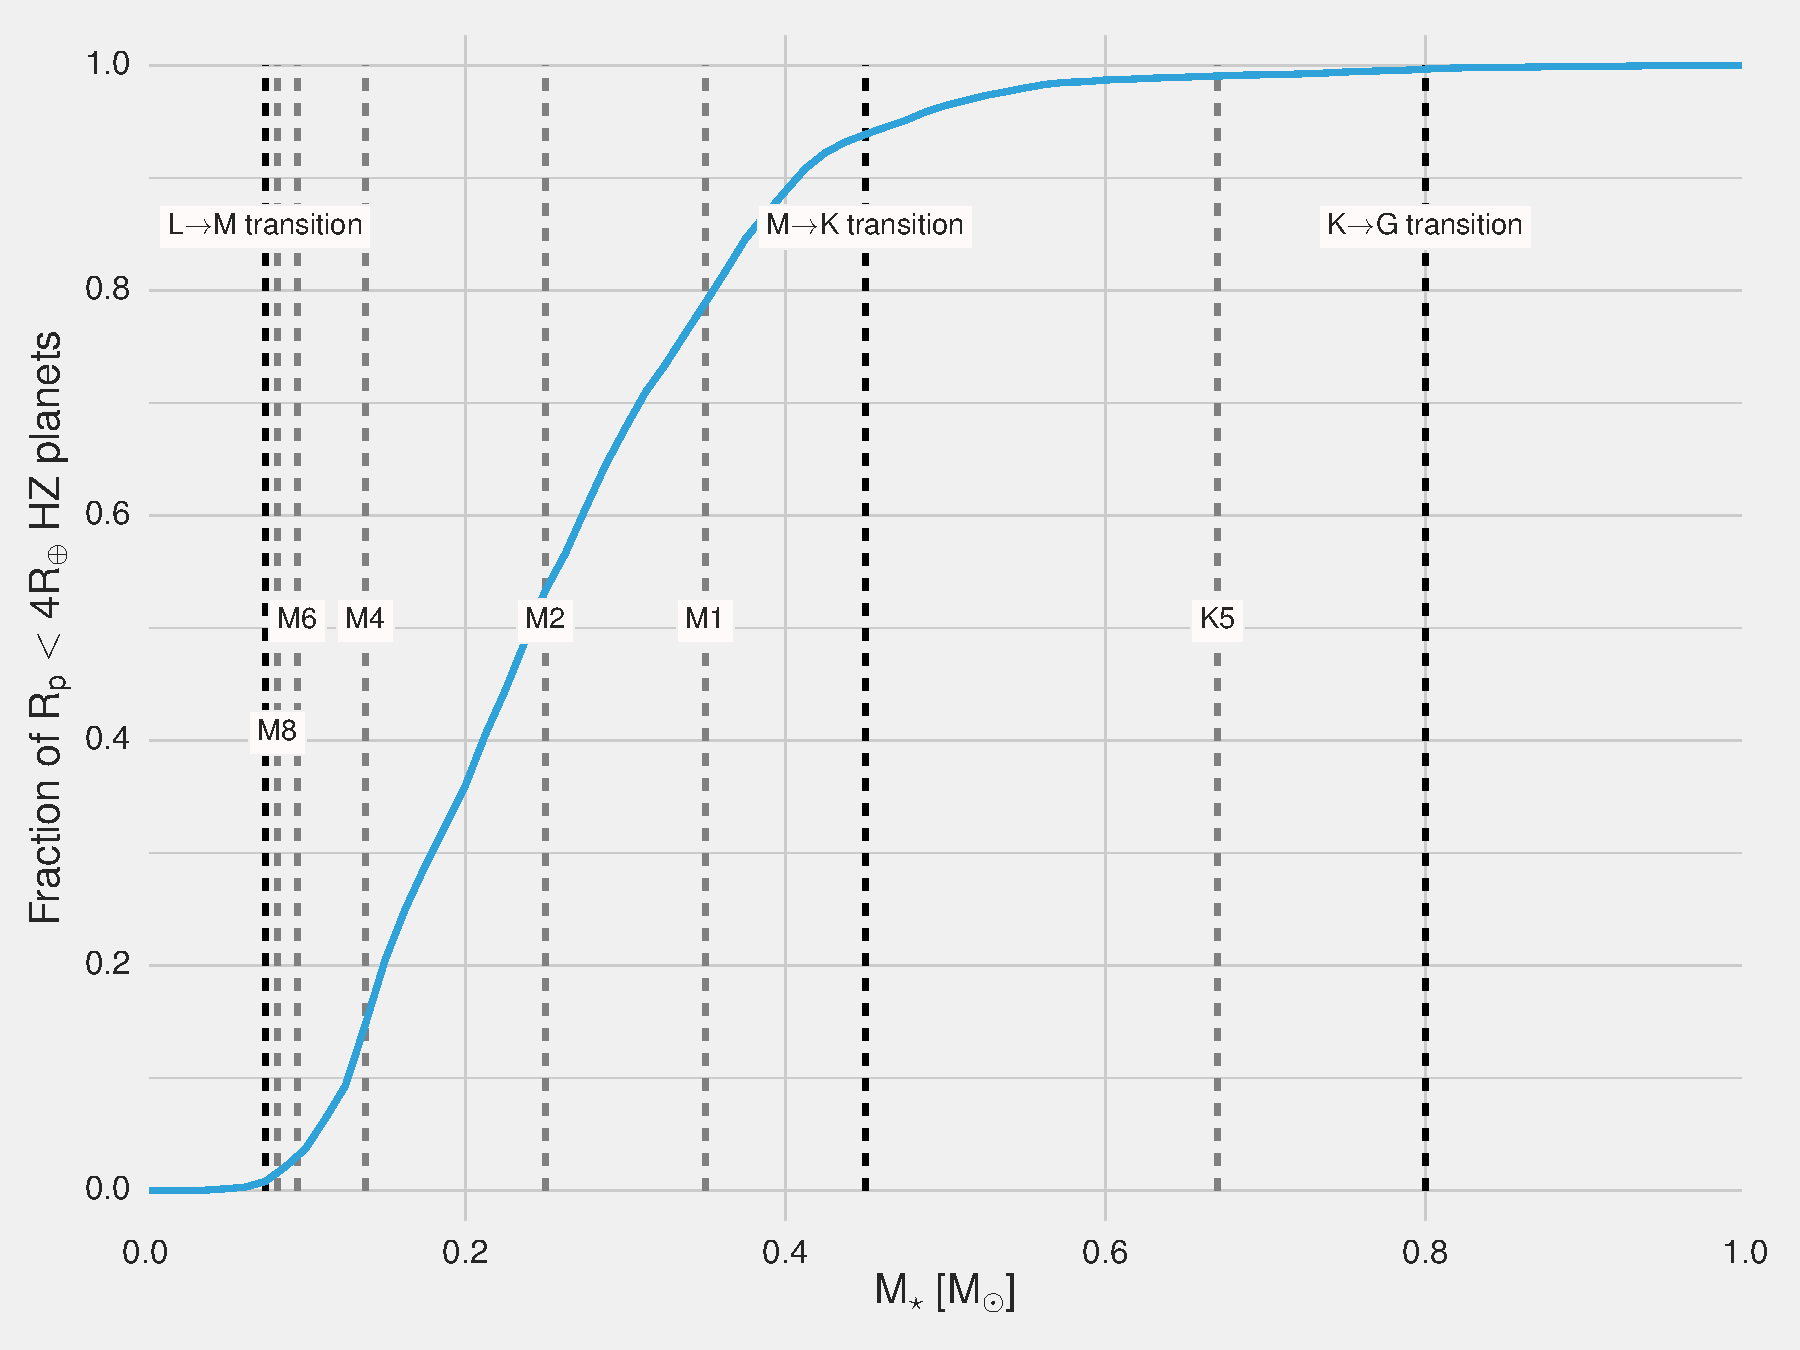
\includegraphics[scale=1.]{figures/CDF_most_HZ_planets_orbit_early_M_dwarfs.pdf}
		\caption{Cumulative distribution of $R_p<4R_\oplus$ and $0.2<S/S_\oplus<2$ planet candidates from the Primary Mission (a proxy for the habitable zone). Boundaries of spectral classes are highly approximate, and taken from from~\protect\citet{habets_empirical_1981} and~\protect\citet{baraffe_massspectral_1996}.}
		\label{fig:CDF_habitable_zone}
	\end{marginfigure}
	\begin{marginfigure}[-1in]
		\centering
		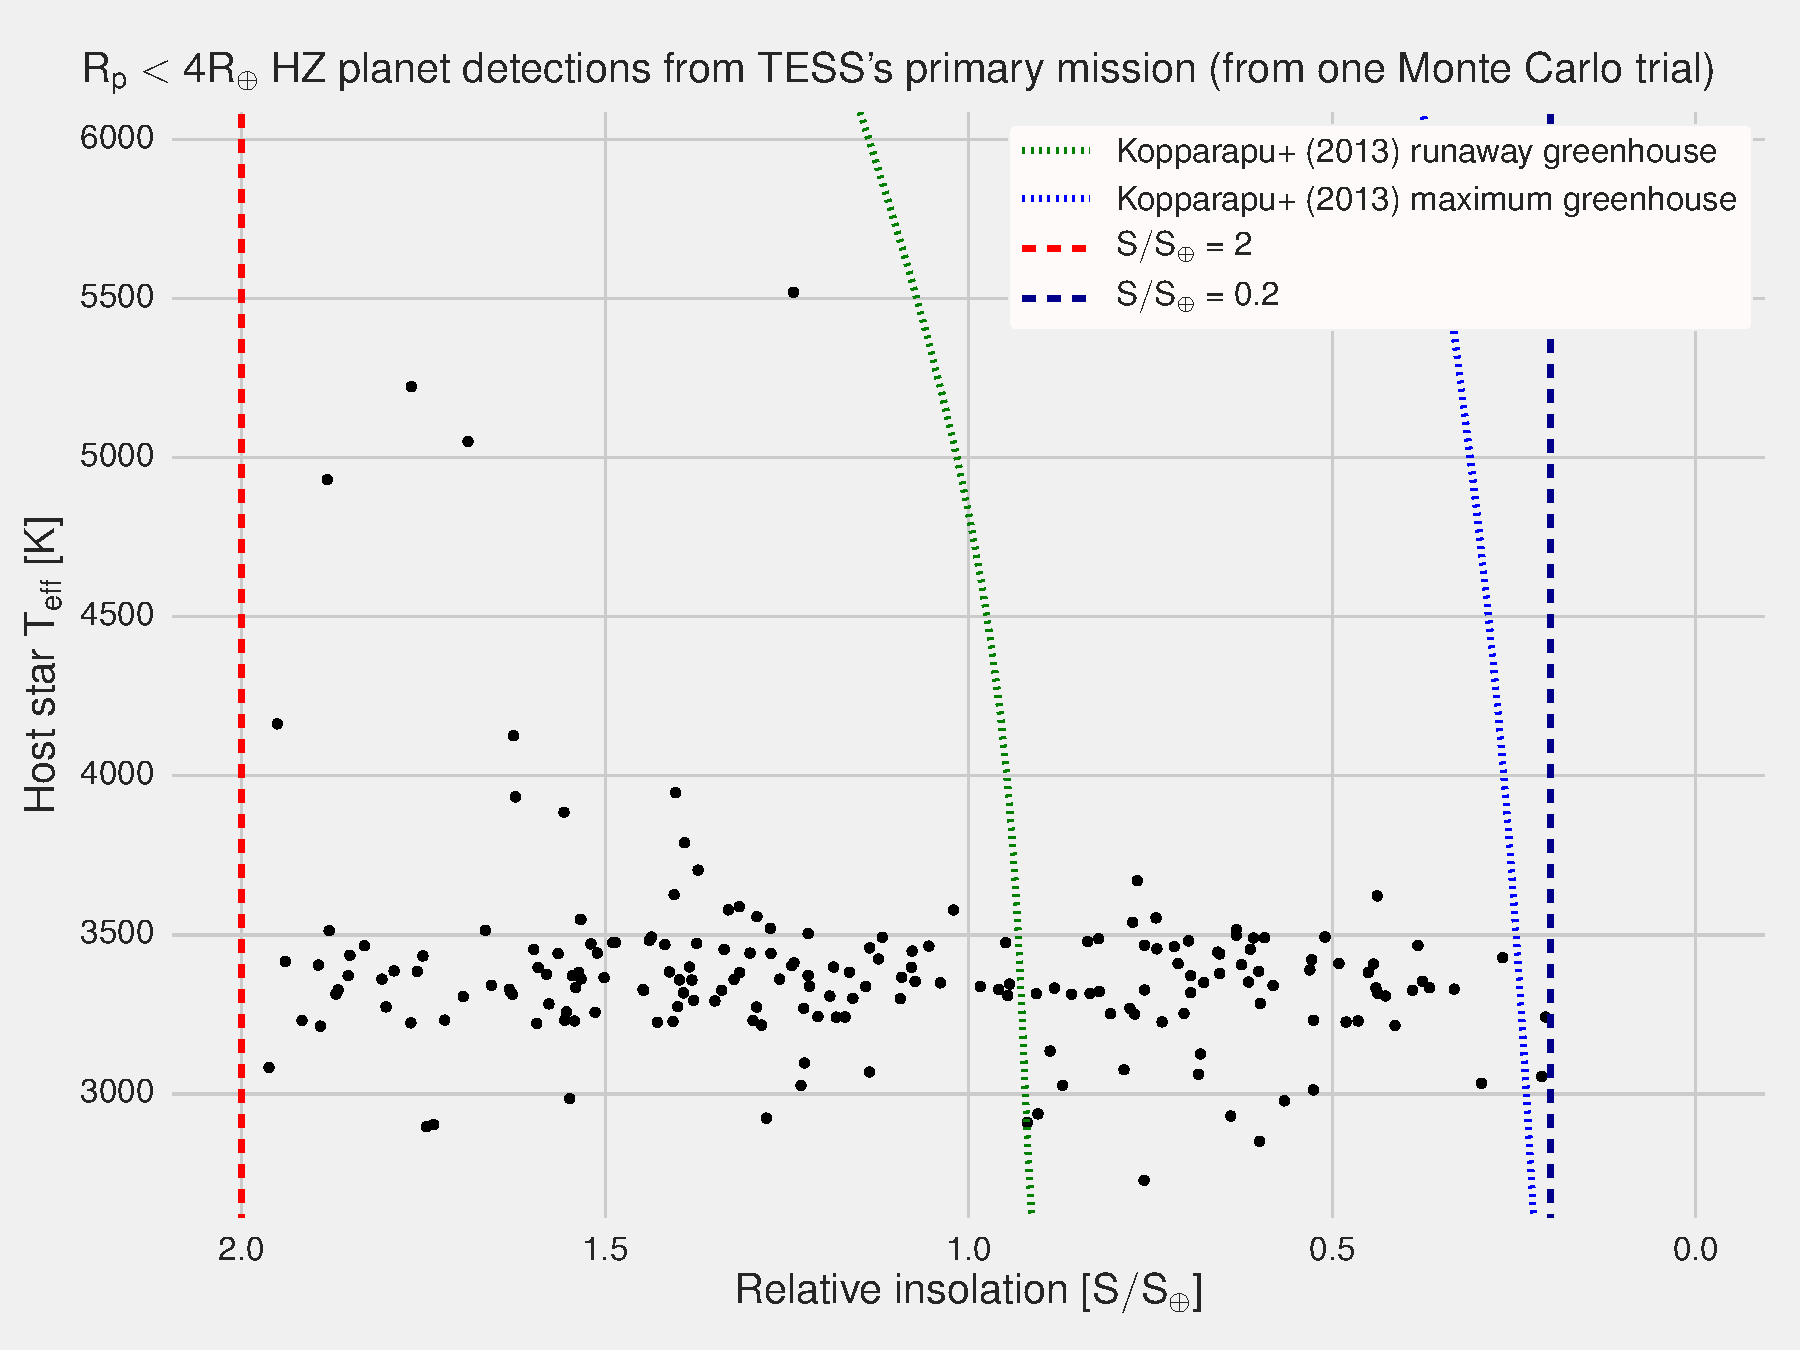
\includegraphics[scale=1.]{figures/hz_planet_detections_rp_lt_4re_kopparapu_2013_incl.pdf}
		\caption{Scatter plot of $R_p<4R_\oplus$ planet candidates falling 
			in the~\protect\citetalias{Sullivan_2015} or 
			\protect\citet{kopparapu_habitable_2013} habitable zones. }
		\label{fig:scatter_habitable_zone}
	\end{marginfigure}	

	\item $N_\mathrm{sys,extra\ planets}$: for how many systems do we detect extra planets?
	Our assumptions about multiple planet system distributions are crude -- we assume independent probability draws from single planet occurrence distributions.
	Thus our simulated planet population may not have systems of tightly packed inner planets in realistic numbers.
	That said, we expect this statistic to be some indication of the information that we are not explicitly modeling, but which can be obtained from extended observations of planetary systems post-planet detection. 
	This additional information includes improved precision on physical and dynamical parameters of the system.
	It also includes transit timing variations, which could be used to discover non-transiting planets as well as transiting outer companions.
	TTVs can also give dynamical hints for the formation history of planetary 
	systems, for instance, discriminating between \textit{in situ} formation 
	and inward migration as~\citet{mills_resonant_2016} argued for the Kepler 
	223 system.

	
	The most prominent feature in the results for this metric is that \elong\:detects the fewest systems with extra planets (44, which is $39\%$ worse than the next-best). 
	This is reasonable because \elong\:spends the most time looking at new sky, and in the process observes fewer systems that were detected in the Primary Mission.
	\nhemi, \shemiAvoid, \npole, and \eshort\:all perform similarly, detecting $\sim65$ such planets.
	\hemis\:detects the most, at 92. While this is still subject to the assumption of two-transit recoverability, in this case the requirement is not too strong: only 10 of \hemis's systems with newly detected planets come from the case where the extra detected planet comes from two transits.
	% makeReport: search for "ntrahemis14d". same for commit.
	
	\item $N_\mathrm{new,atm}$:
	  We define `planets that are amenable to atmospheric characterization' to mean planets whose SNR in transmission is at least half as large as that of GJ~1214b. We chose ``at least half as large'' rather than
          ``equal to'' in order to give a sufficiently large sample to prevent Poisson fluctuations from hindering our comparisons.
	The relevant signal in transmission spectroscopy is the ratio of the areas 
	of atmosphere's annulus to the star's disk on the sky plane, 
	$\delta_\mathrm{atm} = 2\pi R_p h_\mathrm{eff}/(\pi R_\star^2)$, where the 
	effective scale height of the atmosphere $h_\mathrm{eff}$ is proportional to 
	the actual scale height.
	Assuming that the planet is in thermal equilibrium with incident radiation from the host star, and that its atmosphere has known mean molecular weight and Bond albedo, we can compute a representative signal.
	The noise performance depends on the observing instrument, and could be complex if not simply dominated by shot-noise from IR photons.
	We circumvent such complexities via an empirical formula provided to us by Drake Deming, based on a multi-variate regression fit to detailed simulations performed by Dana Louie.
	This formula estimates the SNR in transmission from 4 transits observed with \jwsts NIRISS instrument:
	\begin{align*}
	\log_{10} \mathrm{SNR} =\ &2.98\log_{10}\left(\frac{R_p}{R_\oplus}\right)
							 - 1.019\log_{10}\left(\frac{M_p}{M_\oplus}\right) \\
							 &- 1.459\log_{10}\left(\frac{R_\star}{R_\odot}\right)
							 - 0.249\log_{10}\left(\frac{a}{\mathrm{AU}}\right) \\
							 &- 0.147\left(V - 5.0\right) + 0.193  \numberthis
	\label{eq:atmosphere_Deming}
	\end{align*}
	for $V$ the host star's apparent $V$-band magnitude (calibrated for $3>V>22$), $R_p$ the planet radius, $M_p$ the planet mass, $R_\star$ the star radius, and $a$ the planet's semi-major axis.
	The coefficients are physically sensible: the 2.98 coefficient of $R_p$ minus the 1.019 coefficient of $M_p$ implies that the SNR depends inversely as bulk density, with puffier planets giving higher SNR for transit spectroscopy.
	Although this formula uses a $V$ band magnitude ($\approx$0.5--0.6$\mu$m), while NIRISS's SOSS mode covers 0.6--2.8$\mu$m, the only difference if we were to use $J$ band magnitudes would be in the coefficients preceding the stellar radius and the semi-major axis terms (and thus implicitly, in the stellar mass).
	Focusing our analysis to a SNR measured by \jwst is sensible given \tesss role as a `\jwst finder scope'~\citep{deming_jwst_tess_2009}.
	We focus specifically on NIRISS but our analysis will be broadly applicable 
	to other JWST instruments for transmission 
	spectroscopy (see review by~\citet{beichman_observations_2014}).
	\begin{figure*}[!t]
		\centering
		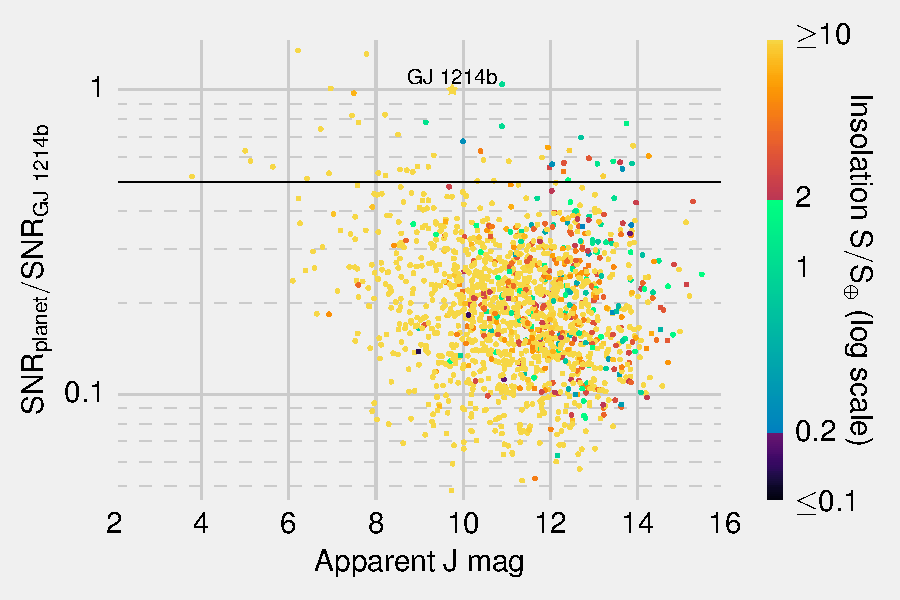
\includegraphics[]{figures/SNR_in_transmission.pdf}
		\caption{ Scatter plot showing the SNR in transmission of detected planets with $R_p<4R_\oplus$ from one Monte Carlo realization of all 3 years of the \npole\:scenario.
			The SNR is computed from Eq.~\protect\ref{eq:atmosphere_Deming}.
			Planets above the horizontal black line ($\mathrm{SNR_{planet}/SNR_{GJ\ 1214b}} = 0.5$) are counted for Fig.~\protect\ref{fig:yield_results}'s metric of planets with `good' atmospheres for transmission spectroscopy.
			GJ 1214b is marked with a star.
			The coloring of planets indicates their relative insolation, as well as 
			whether they are in our approximate habitable zone ($0.2<S/S_\oplus<2)$.
		}
		\label{fig:atmosphere_scatter}
	\end{figure*}

	The system values for GJ 1214b are those found
	by~\citet{charbonneau_gj1214b_2009}: $R_p = 2.678R_\oplus$, $M_p = 6.55M_\oplus$,
	$R_\star = 0.211R_\odot$, $a = 0.0144\mathrm{AU}$, $V = 15.1$.
	Using Eq.~\ref{eq:atmosphere_Deming}, we compute the SNR in transmission for 
	all detected planets, for all Extended Mission scenarios.
	We normalize them to the equivalent SNR for GJ 1214b (3.94, per 
	Eq.~\ref{eq:atmosphere_Deming}).
	Fig.~\ref{fig:atmosphere_scatter} shows one realization of the resulting 
	distribution for planets detected in all three years of the \npole\:scenario.

	\tess mostly detects strongly irradiated planets (most points on Fig.~\ref{fig:atmosphere_scatter} are yellow).
	A very small number, $\lesssim 10$, are both in the approximate habitable zone and also `favorable for atmospheric characterization'.
	Of course, a highly compelling target with lower SNR in transmission per transit might merit a more ambitious \jwst observing program.
	We note that all of these planets are assumed to have identical mean molecular weights and cloud properties.
	%\todo[inline]{what cloud model/opacity does this use?}

	More importantly, Fig.~\ref{fig:yield_results} shows that most of the planets with atmospheres that are best for transmission spectroscopy are already discovered after two years.
	The best Extended Missions (\shemiAvoid, \elong, \eshort\:and \hemis) boost 
	the yield of such planets from $\sim\!100$ ($N_\mathrm{pri,atm}$) to 
	$\sim\!120$ ($N_\mathrm{pri,atm} + N_\mathrm{new,atm}$).
	The worst, \npole, finds about an additional 10.
	This best-case boost of $1.25\times$ more `good' planets for atmospheric characterization is less than the relative boost of $1.6\times$ more newly detected long period planets.
	Put differently, among the various possibilities for the Extended Mission,
        there is more variation in $N_\mathrm{new,P>20d}$ than in 
        $N_\mathrm{new,atm}$.
	
	
	\item $N_\mathrm{new,new\ stars}$:
	  Intuitively we expect that to maximize the number of planets detected 
	  around ``new'' stars (those which were not observed during the Primary 
	  Mission) we should collect as many photons as possible from new stars.
         And the region on the sky with the greatest number of new stars is the ecliptic.
	 It is not surprising, then, that the \elong\:scenario finds the largest number of planets around new stars.
         The \elong\:scenario dedicates 7 of a single year's 13 observing sectors to the ecliptic (where the other 6 are spent centered at the North Ecliptic Pole due to excessive Earth and Moon crossings).
	It consequently detects twice as many new planets about newly observed 
	stars as the next-best scenarios: \eshort\:and \shemiAvoid\:(366 vs 171 and 
	114, respectively).
	These latter two scenarios also spend time observing the ecliptic, but with 
	only one camera, rather than with all four cameras simultaneously.
	We note that even though \elong\:is the scenario most successful in 
	detecting planets about new stars, the new stars represent only 
	$\sim\!30\%$ of the total number of new detections.\footnote{Here, we 
	remind the reader that ``new'' refers only to \tess observations. Some of 
	these stars will
          have been observed by K2 or other projects (see discussion in Sec.~\ref{sec:discussion}).}

	\item $N_\mathrm{new,SNR\lor N_{tra}}$:
	This statistic is the number of newly detected planets that are detected either (a) due to their final SNR clearing our threshold (logical) or (b) their number of observed transits being greater than or equal to 2.
	It is the complement to $N_\mathrm{new,new\ stars}$: scenarios like \nhemi, \npole, and \hemis\:that do not observe many new stars will detect all of their planets from a boosted SNR and/or clearing the minimum transit threshold.
	
\end{enumerate}

\paragraph{Comment on meaning of `detected in postage stamps' vs `detected in FFIs'}
The invested reader may inquire ``what about the cross-over case of planets that are observed as PSs during the Primary (Extended) Mission, but as FFIs in the Extended (Primary) Mission? These are not explicitly listed in Fig.~\ref{fig:yield_results}''.
%This is what is done in Fig.~\ref{fig:yield_results}.
When describing the entire unique planet population detected from Years 1-3, for simplicity of language we use `postage stamp detections' to refer to planets that are observed at any time (Primary or Extended Missions) at 2 minute cadence.
In these cases, the dominant contribution to the final signal to noise ratio tends to come from the PS observations.
When describing new planet detections, we use `postage stamp detections' to mean planets that were newly detected due to being observed as postage stamps in the Extended Mission.
In other words, this `cross-over' point only matters in discussions of the unique planet population from an entire mission, Years 1-3.
Considering just the newly detected planet population, we can unambiguously specify whether the new detections came from full frame images or postage stamps, irrespective of their observations from the Primary Mission.
